% !TeX root = POSTER.tex
\documentclass[25pt, a0paper,
portrait,
% landscape,
margin=5mm, innermargin=5mm, blockverticalspace=15mm, colspace=15mm, subcolspace=0mm]{tikzposter}
		
% -- Packages --------------------------------------------------------%
\usepackage{amsfonts,amssymb,amsmath,mathtools}
\usepackage{defcmlfont}
\usepackage{tikz,lipsum}
\usetikzlibrary{positioning}
\usepackage{float}                           % for minipages at Polarization part
\usepackage{caption}                         % no "Figure" in caption
\captionsetup[figure]{labelformat=empty}

\usepackage{psfrag}

% Load figures command: \inputfig [htb]{fig_dir}{fig_label}
\newcommand*{\inputfig}[3][htb]{{
    \def\fps@figure{#1}
    \def\DIR{#2}
    \def\LABEL{#3}
    \graphicspath{{\DIR/}}
    \psfrag{sm}[c][c]{\small \textsc{Scan me}}


\includegraphics[width=0.03\textwidth]{QRcode_ACoM.eps}
}}

\usepackage{fontawesome}
\usepackage{bm}
\usepackage{bigints}

% -- Commands --------------------------------------------------------%
% \newcommand{\wall}{\text{w}}
% \newcommand{\interf}{\text{i}}
% \newcommand{\phase}{k}	
% \newcommand{\liquid}{\ell}
% \newcommand{\steam}{g}
% \newcommand{\out}{\text{out}}
% \newcommand{\tr}{{\mathsf T}}
\newcommand{\WAsigma}{\prescript{\prescript{\mathcal{W}}{}{\!\!\!\mathcal{A}}}{}{\!\sigma}}
\newcommand{\WABsigma}{\prescript{\prescript{\mathcal{W}}{}{\!\!\!\mathcal{A}}}{}{\!\boldsymbol{\sigma}}}

% -- Title, Author, Institute --------------------------------------------------------%
\title{\bfseries Mathematical modelling for the next-generation all-solid-state battery: \\
\bfseries Nucleation interface}
% \author{Tuan Vo$^{\text{(1),(2)}}$}
\author{Tuan Vo}
\institute{
	ACoM, Applied and Computational Mathematics, RWTH Aachen University
% (2) IEK-2, Institute of Energy and Climate Research, Forschungszentrum Jülich
}
% \titlegraphic{
\includegraphics[height=6cm]{./figs/FZJ_only.pdf} \hfill 
\includegraphics[height=6cm]{./figs/rwth_mathcces_bild_rgb_only.pdf} }
\titlegraphic{
\includegraphics[width=0.4\textwidth]{./floats/logos/rwth_acom_en_cmyk.eps}}

\renewcommand{\familydefault}{\sfdefault}

\bibliographystyle{plain}

\newcommand{\newcaption}[2]{\parbox{#1}{\centering{\small \it #2\par}}\normalsize}

% -- Predefined Colors and Themes ---------------------- %
% Choose THEME:  Default, Basic, Rays, Simple, Envelope, Wave, Board, Autumn, Desert,
\usetheme{Simple}

\useblockstyle[titleinnersep=5mm]{Default}    % change default parameter for title inner sep

% Choose COLOR STYLE:  Default, Blue, BlueGray, BlueOrange, BlueViolet, DarkBlue, GrayBlue, GrayLightblue, GrayRed, Green, GreenOrange, YellowRed
%\definecolor{main}{HTML}{0080FF}
%\definecolor{sub}{HTML}{8CDBFF}
%\usecolorstyle[colorOne=sub, colorTwo=main]{Default}
     
% ---------------------------------------------------------------------------------------------------------------- %
\begin{document}

% Title block
\maketitle[width=750mm]
% ---------------------------------------------------------------------------------------------------------------- %
\begin{columns}

	% FIRST column
	\column{0.515}
	% ---------------------------------------------------------------------------------------------------------------- %
	\block{Next-generation All-solid-state battery}{
	Rechargeable Lithium-ion battery (LIB) stays at the heart of every energy storage system and electric vehicle. 
	Undoubtedly, LIB benefits human life efficiently as well as friendly-environment. 
	Besides, a more advanced LIB, so-called \textbf{all-solid-state battery} (ASSB), 
	is introduced recently  as ASSB is expected with non-inflammation and non-explosion as seen in common LIBs. 
	Yet, defect due to polarization is one natural phenomenon of \textbf{solid electrolyte} (SE) to be tackled.\\
	[0,5em]
	This poster is aimed to model the polarized SE with the use of \textbf{structural tensor}.
	% \begin{center}
	% \fbox{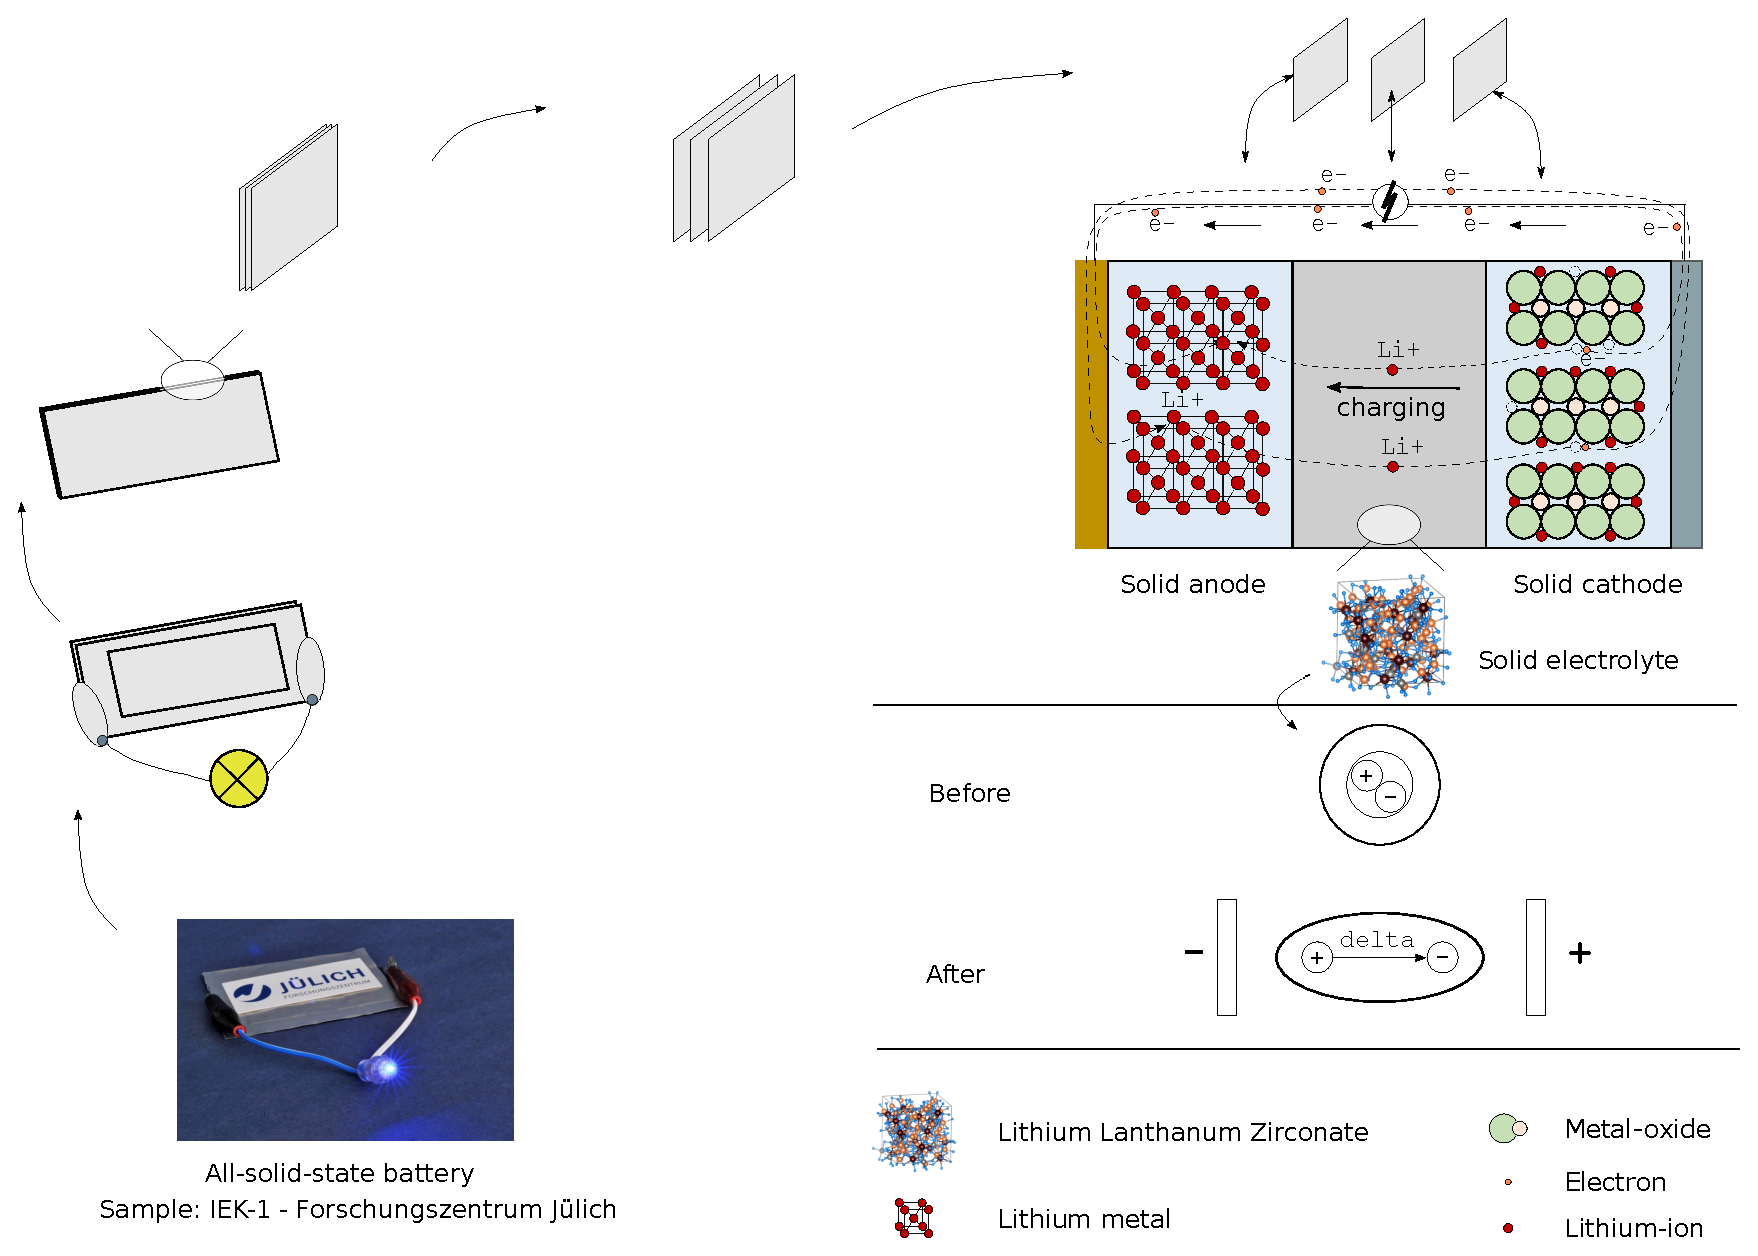
\includegraphics[height=18cm]{./figs/dendrite/dendritetext}}
	% \fbox{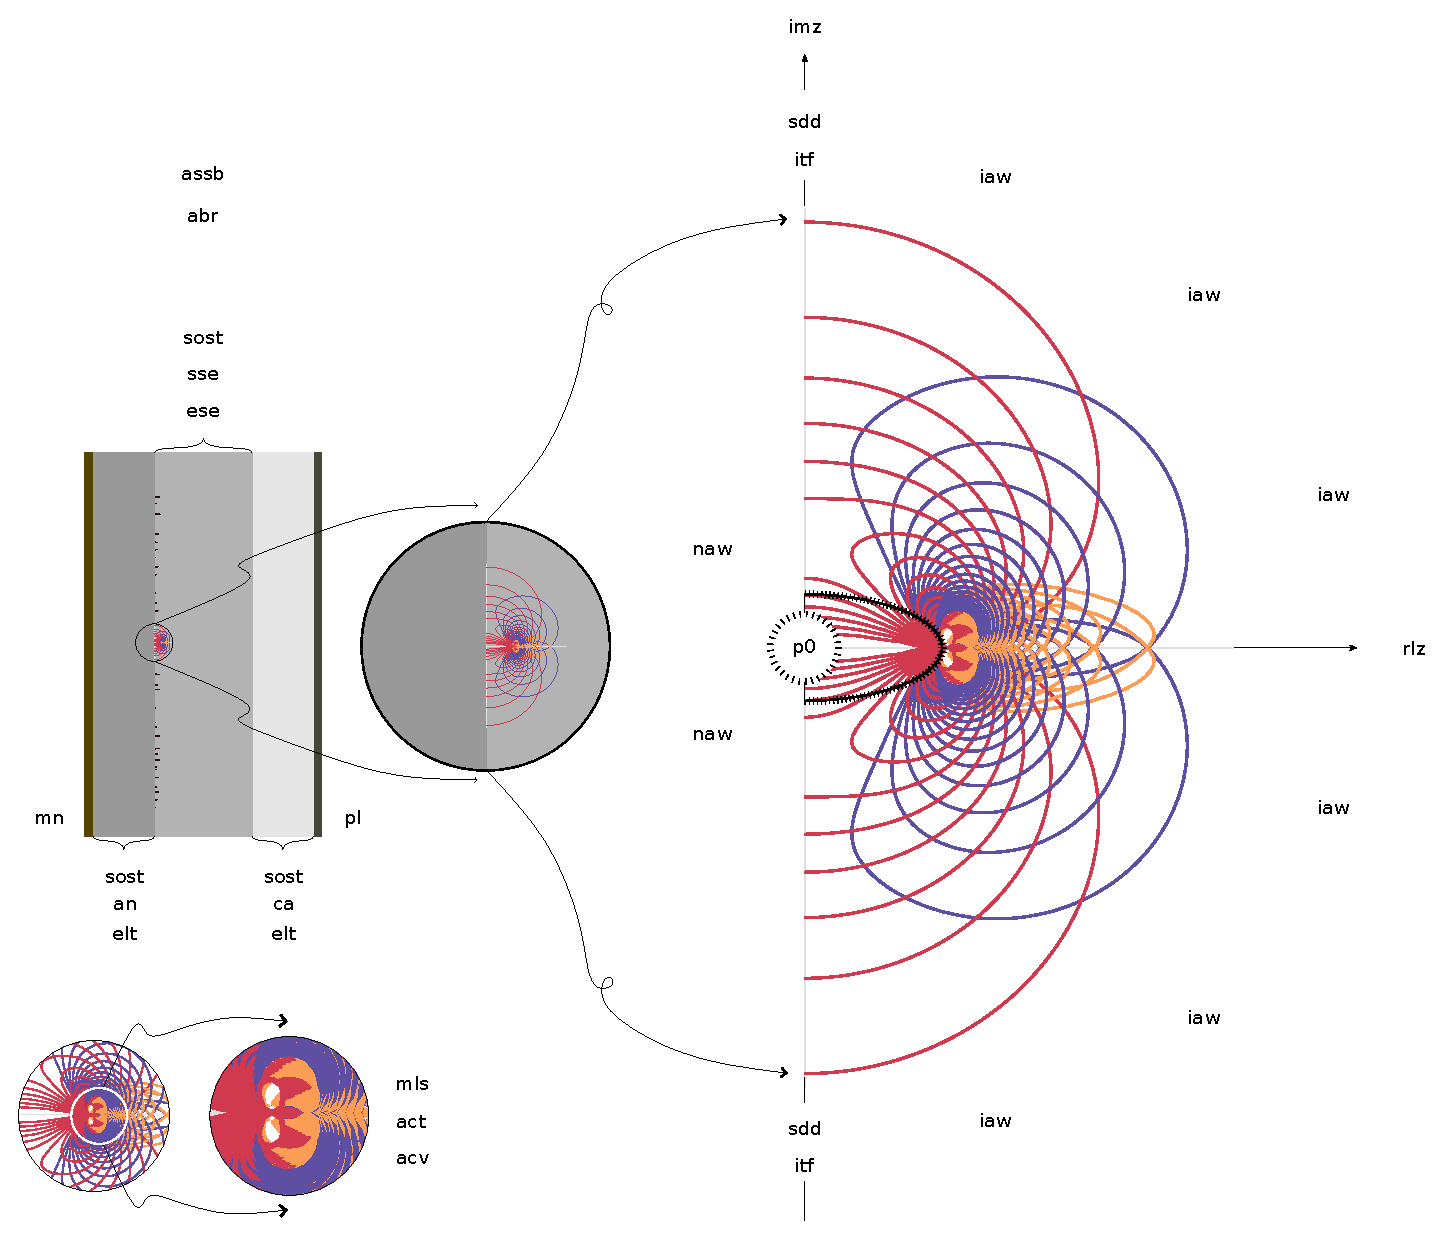
\includegraphics[height=18cm]{./floats/creviceAiryWestergaard_compare/creviceAiryWestergaard_compare.eps}}
	% 	\newcaption{0.8\colwidth}{A sample of a typical all-solid-state battery and its non-scale hierarchical insight into structural layers.}
	% \end{center}
	A typical LIB includes three main components: cathode, anode and electrolyte. 
	Different types of LIB have a variation of constitutive material composed of battery. 
	An ASSB means that the three main components are \textbf{all made of solid material}.
	\begin{center}
		% \fbox{\inputfig{floats/creviceAiryWestergaard_compare}{creviceAiryWestergaard_compare}}
		\inputfig{floats/creviceAiryWestergaard_compare}{creviceAiryWestergaard_compare}
	\end{center}
	}
	% ---------------------------------------------------------------------------------------------------------------- %
	\block{Modelling goal: Interface analysis + Numerical modelling}{
		Two main goals to model the solid electrolyte part of the all-solid-state battery is as follows:
		%
		\begin{enumerate}
			\item To capture the \textbf{preferred direction} behaviour of the solid electrolyte due to electric potential.
			\item To satisfy \textbf{thermodynamic consistency}%\cite{braun2015SCL}
			      :
			      \begin{itemize}
				      \item Conservation of mass, linear $\&$ angular momentum and energy for the solid electrolyte.
				      \item Entropy inequality is guaranteed with sharper conditions, which lead to constitutive equation.
			      \end{itemize}
		\end{enumerate}
		\begin{align*}
			a_{\text{Griffith}}:= a^{*}
			= \arg\min_{a\in\mathbb{R}}
			{
				\bigintsss\!\!\!\!\!\!\bigintsss\!\!\!\!\!\!\bigintsss_{\Omega}
				f(a,\bm{u};\lambda,\mu,\bm{d}\otimes\bm{d}) \, d\Omega
				-
				\bigintsss\!\!\!\!\!\!\bigintsss_{\Gamma}
				f(a;\gamma) \, d\Gamma
			}\Bigg|_{\bm{u}^{(s)}}
		\end{align*}
	}
	% ---------------------------------------------------------------------------------------------------------------- %
	% \block{Continuum physics kinematic}{
	% 	Green-Lagrange strain tensor $\BE$ with respect to \textbf{small} displacement 
	% 	$\partial\Bu/\partial\Bxi = \mathcal{O}(\epsilon), \ \epsilon \ll 1$:
	% 	\begin{align*}
	% 		\BE = \frac{1}{2}(\BF^{\top}\BF -\BI) =\frac{1}{2}\left(
	% 		\frac{\partial\Bu}{\partial\Bxi} + \left( \frac{\partial\Bu}{\partial\Bxi} \right)^{\top}
	% 		+\underbrace{\left( \frac{\partial\Bu}{\partial\Bxi} \right)^{\top}\left( \frac{\partial\Bu}{\partial\Bxi} \right)}_{\text{Neglected}}
	% 		\right) \ \rightarrow \
	% 		\Bvarepsilon := \frac{1}{2}\left(
	% 		\frac{\partial\Bu}{\partial\Bxi} + \left( \frac{\partial\Bu}{\partial\Bxi} \right)^{\top}\right)
	% 	\end{align*}
	% }
	% ---------------------------------------------------------------------------------------------------------------- %	
	% \block{Polarization phenomenon}{
	% 	Due to a source of electric potential pointing from cathode $(+)$ to anode $(-)$ pole, 
	% 	a uniform electric field created has suppressed on 
	% 	the SE occupied between these two poles. Consequently, SE yields to a \textbf{preferred direction}
	% 	under external deformations such as mechanical loading forces.
	% 	% \begin{minipage}{\linewidth}
	% 	% 	\centering
	% 	% 	\begin{minipage}{0.20\linewidth}
	% 	% 		\begin{figure}[H]
	% 	% 			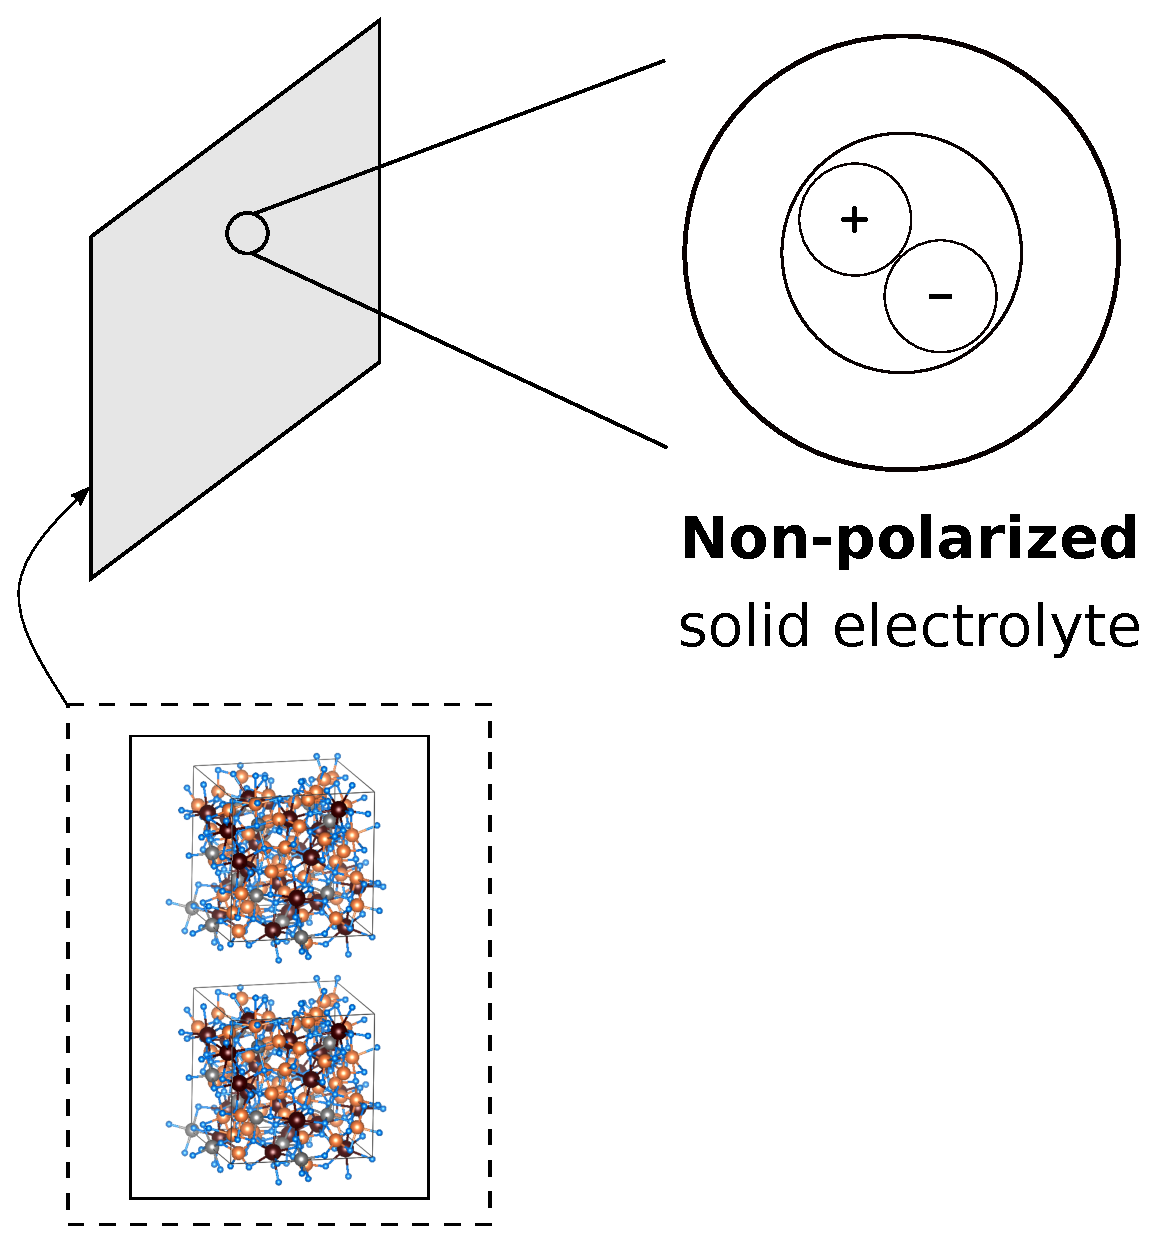
\includegraphics[width=\linewidth]{./figs/polarization/polarizedSEnon}
	% 	% 			%\caption{Non-polarized SE.}
	% 	% 		\end{figure}
	% 	% 	\end{minipage}
	% 	% 	\hspace{0.2\linewidth}
	% 	% 	\begin{minipage}{0.25\linewidth}
	% 	% 		\begin{figure}[H]
	% 	% 			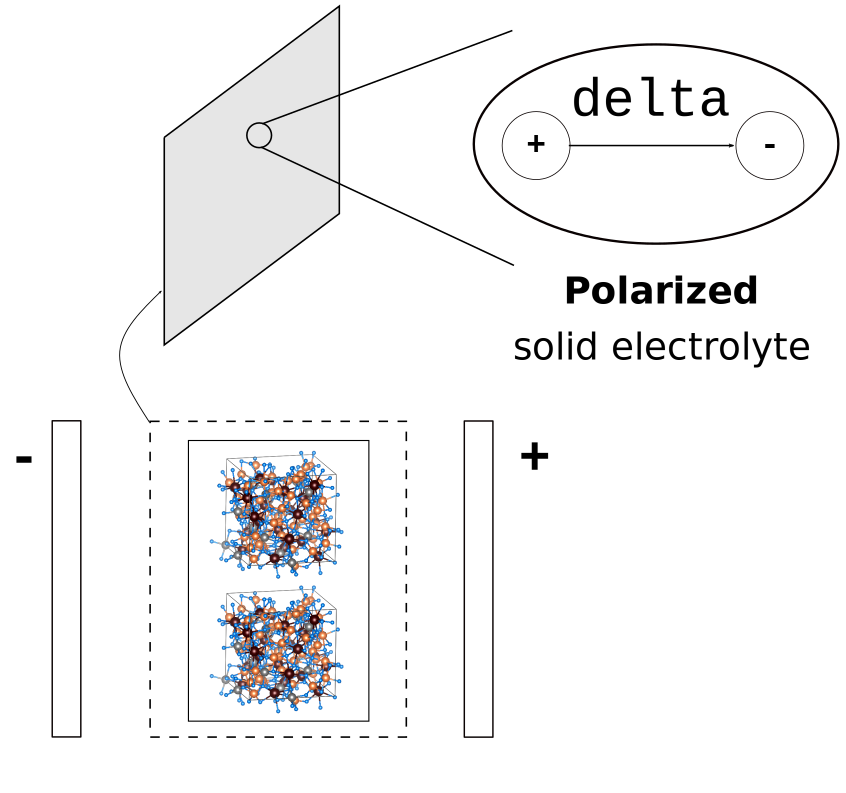
\includegraphics[width=\linewidth]{./figs/polarization/polarizedSE}
	% 	% 			%\caption{Polarized SE.}
	% 	% 		\end{figure}
	% 	% 	\end{minipage}
	% 	% \end{minipage}
	% }
	% ---------------------------------------------------------------------------------------------------------------- %	
	\block{Contact}{
		{
				\raggedleft
				\begin{tikzpicture}
					\node (qrcode)
					{
						\inputfig{floats/QRcode_ACoM}{QRcode_ACoM}
						% 
\includegraphics[width=3cm]{./floats/QRcode_ACoM/QRcode_ACoM.eps}
					};
					\node [left= 0mm of qrcode.north west, yshift=-25mm]
					{
						% \hspace{0mm} 
						Tuan Vo 
						$\cdot$ ACoM 
						$\cdot$ RWTH Aachen University 
						$\cdot$ Email: vo@acom.rwth-aachen.de};
				\end{tikzpicture}
			}
		% \inputfig{floats/QRcode_ACoM}{QRcode_ACoM}
		% Tuan Vo $\cdot$ RWTH Aachen University $\cdot$ Email: vo@acom.rwth-aachen.de
	}
	% ---------------------------------------------------------------------------------------------------------------- %
	% ---------------------------------------------------------------------------------------------------------------- %
	% ---------------------------------------------------------------------------------------------------------------- %
	% ---------------------------------------------------------------------------------------------------------------- %
	% ---------------------------------------------------------------------------------------------------------------- %
	% SECOND column
	% ---------------------------------------------------------------------------------------------------------------- %
	% ---------------------------------------------------------------------------------------------------------------- %
	% ---------------------------------------------------------------------------------------------------------------- %
	% ---------------------------------------------------------------------------------------------------------------- %
	% ---------------------------------------------------------------------------------------------------------------- %
	% \column{0.485}
	% \block{Mathematical model}{
	% 	\textbf{Constitutive equation} is first derived from considering local balance laws and enforcing sharper conditions to entropy inequality.
	% 	\begin{itemize}
	% 		\item Local balance laws governing the infinitesimal elasticity embedded structural tensor:
	% 		      \begin{align*}
	% 			       & \text{Balance of mass}             &  & \dot{\rho} + \rho{\ \rm div}\Bv = 0                             \\
	% 			       & \text{Balance of linear momentum}  &  & \rho\dot{\Bv} = {\rm div}\Bpi + \rho\Bb                         \\
	% 			       & \text{Balance of angular momentum} &  & \Bpi^{\top} = \Bpi                                              \\
	% 			       & \text{Balance of energy}           &  & \rho\dot{e} = \Bpi : \dot{\Bvarepsilon} + \rho r - {\rm div}\Bq
	% 		      \end{align*}
	
	% 		\item Entropy inequality
	% 		      \begin{align*}
	% 			      \rho\calD := \Bpi :\dot{\Bvarepsilon}  -\rho\eta\dot{\theta}- \rho\dot{\Psi} -\frac{1}{\theta}\Bq\cdot\nabla\theta \geq 0 
	% 		      \end{align*}
	
	% 		\item Mathematical model:
	% 		      \begin{align*}
	% 			       & \text{PDE}                   &  & \pi_{ij,j} + \rho b_{i} = 0                                                                                      \\
	% 			       & \text{Kinematic relation}    &  & \varepsilon_{kl} = \frac{1}{2}\left(\frac{\partial u_k}{\partial x_l} + \frac{\partial u_l}{\partial x_k}\right) \\
	% 			       & \text{Constitutive relation} &  & \pi_{ij} = \mathbb{C}_{ijkl}\ \varepsilon_{kl}                                                                   \\
	% 			       & \text{Dirichlet BC}          &  & u_i = \bar{u}_i \text{ on } \partial\Omega_{u_i}                                                                 \\
	% 			       & \text{Neumann BC}            &  & \pi_{ij}n_j = t_i \text{ on } \partial\Omega_{t_i}
	% 		      \end{align*}
	% 		      %
	% 		      \begin{align*}
	% 			      \begin{aligned}
	% 				      \text{where } \qquad 
	% 				      \mathbb{C}_{ijkl} & = \lambda \delta_{ij}\delta_{kl} + 2\mu_T\mathbb{I}_{ijkl}     \\
	% 				                        & + \alpha(\delta_{ij}M_{kl} + M_{ij}\delta_{kl})
	
	% 				      + 2(\mu_L-\mu_T)\left[\mathbb{I}_{\Bd}\right]_{ijkl} + \beta M_{ij}M_{kl}          \\
	% 				      \left[\mathbb{I}_{\Bd}\right]_{ijkl}
	% 				                        & = \frac{1}{2}(d_{i}\delta_{jl}d_{k} + d_{i}\delta_{jk}d_{l}
	
	% 				      +d_{j}\delta_{ik}d_{l} + d_{j}\delta_{il}d_{k})                                    \\
	% 				      \mathbb{I}_{ijkl} & = \frac{1}{2}(\delta_{ik}\delta_{jl} + \delta_{il}\delta_{jk})
	% 			      \end{aligned}
	% 		      \end{align*}
	% 	\end{itemize}
	% }
	% % ---------------------------------------------------------------------------------------------------------------- %	
	% \block{Structural tensor}{
	% 	SE microstructure with structural tensor $\BM = \Bd \otimes \Bd$ is defined by a symmetry group $\mathbb{G}$:
	% 	\begin{align*}
	% 		\mathbb{G} := \left\{ \BQ_{||_{\Bd}}, \BQ_{\bot_{\Bd}}  \right\} \subset \mathcal{O}(3),
	% 	\end{align*}
	% 	which leads to invariant free energy function $\hat{\Psi}$ under rotations followed by group $\mathbb{G}$:
	% 	\begin{align*}
	% 		\hat{\Psi}(\Bvarepsilon,\BM) = \hat{\Psi}(\BQ\Bvarepsilon\BQ^{\top},\BQ\BM\BQ^{\top}) = \hat{\Psi}(\Bvarepsilon,\BM)  \quad \forall \ \BQ \in \mathbb{G}.
	% 	\end{align*}
	% }
	% % ---------------------------------------------------------------------------------------------------------------- %	
	% \block{Next steps and future direction}{
	% 	\begin{itemize}
	% 		\item Time-dependent implementation, numerical analysis, verification and validation.
	% 		\item Explicit description of coordinate-based polarization variation.
	% 		\item Bridging scale into quantum physics: Update information from quantum for continuum.
	% 		\item Capture a phenomenon so-called \textbf{dendrite formation}:
	% 		    %   \begin{center}
	% 			%       %\vspace*{1em}
	% 			%       \fbox{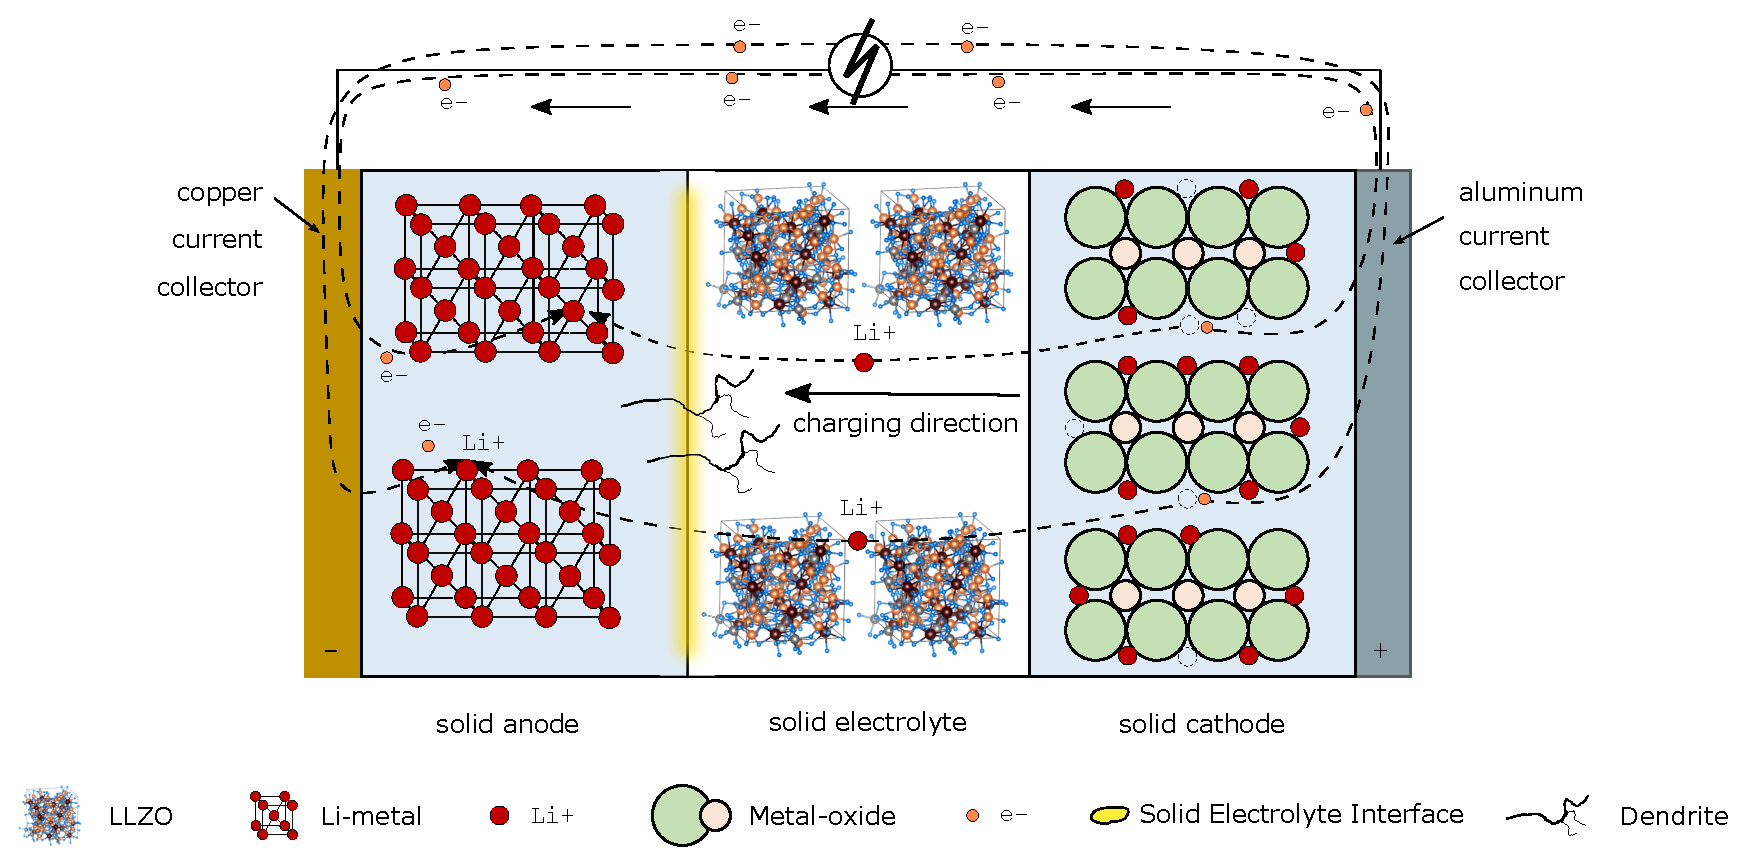
\includegraphics[width=28cm]{./figs/transport/transporttext}}\vspace*{1em}
	% 			%       \newcaption{0.8\colwidth}{Dendrite formation: After a several number of charging cycles, dendrite branches are slowly formed and developed from Solid electrolyte interface (SEI) through grain boundaries.}
	% 		    %   \end{center}
	% 	\end{itemize}
	% }
	% % ---------------------------------------------------------------------------------------------------------------- %	
	% \block{References}{
	% 	\vspace*{-3em}
	% 	\renewcommand{\refname}{~}
	% 	\begin{thebibliography}{2}
	
	% 		\bibitem{viozat1997implicit}
	% 		Vo T. \emph{Modeling the swelling phenomena of lithium-ion battery cells based on a numerical chemo-mechanical coupled approach}. 
	% 		Master thesis, 2018.
	
	% 		\bibitem{braun2015SCL}
	% 		S. Braun, C. Yada and A. Latz. \emph{Thermodynamically consistent model for Space-Charge-Layer formation in a solid electrolyte}. 
	% 		Journal of Physical Chemistry, 119, 22281-22288, 2015.
	
	% 	\end{thebibliography}
	% }
\end{columns}

\end{document}
% ---------------------------------------------------------------------------------------------------------------- %